\iffalse
%\documentclass{article}
\documentclass[journal,12pt,twocolumn]{IEEEtran}

% Language setting
% Replace `english' with e.g. `spanish' to change the document language
\usepackage[english]{babel}

% Set page size and margins
% Replace `letterpaper' with `a4paper' for UK/EU standard size
%%\usepackage[letterpaper,top=2cm,bottom=2cm,left=3cm,right=3cm,marginparwidth=1.75cm]{geometry}

% Useful packages
\usepackage[utf8]{inputenc}
\usepackage{enumitem}
\usepackage{multicol}
\usepackage{ragged2e}
\usepackage{amsmath}
\usepackage{amssymb}
\usepackage{graphicx}
\let\vec\mathbf
\let\myvec\bf
\usepackage{array}
\usepackage{blindtext}
%\usepackage[paperwidth=10cm]{geometry}
\usepackage{tkz-euclide}
%\usepackage{tikz}
\usetikzlibrary{
  circuits.logic,
  circuits.logic.US,
  positioning
}
\usepackage[colorlinks=true, allcolors=blue]{hyperref}

\title{Line Assignment}
\author{Navya Valmeekam}
\let\vec\mathbf
\begin{document}
\providecommand{\norm}[1]{\left\lVert#1\right\rVert}
\maketitle
\begin{tableofcontents}
\section{Problem}
\fi
In figure below, $ABCD$ is a parallelogram and $BC$ is produced to a point $\vec{Q}$ such that $AD = CQ$. If $AQ$ intersect $DC$ at $\vec{P}$, show that 
	\begin{align}
	ar (BPC) = ar (DPQ).
		\label{eq:9/9/4/4}
	\end{align}
	\begin{figure}[H]
		\centering
 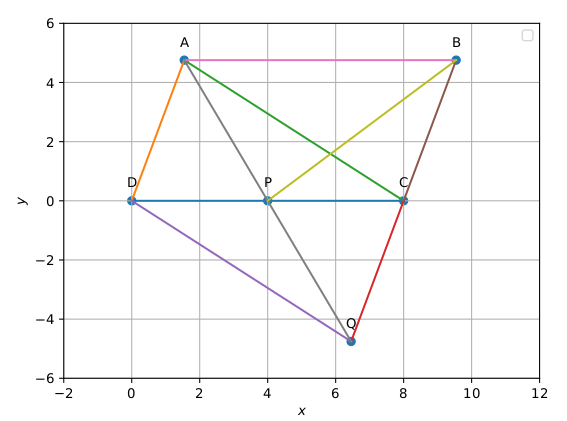
\includegraphics[width=0.75\columnwidth]{chapters/9/9/4/4/figs/construction.png}
		\caption{}
		\label{fig:9/9/4/4}
  	\end{figure}
	\iffalse
[Hint : Join AC.]\\
\includegraphics[scale=0.4]
\begin{center}
Figure of Construction
\end{center}
\section{Construction}
\begin{center}
\begin{tabular}{|c|c|c|}
\hline
\textbf{Symbol}&{Value}&{Description}\\
\hline
r1&5&DA\\
\hline
r2&8&DC\\
\hline
${\theta}_1$& 2$\pi/5$&$ \angle $ADC\\ 
\hline
\end{tabular}
\end{center}
\begin{center}
\begin{equation}
\vec{B}= \vec{A}+\vec{C}-\vec{D}
\end{equation}
\begin{equation}
\vec{Q}= \vec{D}+\vec{C}-\vec{A}
\end{equation}
\begin{equation}
\vec{P}= \vec{(D+C)/2}
\end{equation}
\end{center}
%\end{abstract}
\section{Solution}
\justify
\textbf{Construction: Join AC}\\
\justify
\textbf{To Prove:}
ar($\Delta$ BPC) = ar($\Delta$ DPQ)\\
\\
We need to prove that ar(BPC)=ar(DPQ)\\
\\
Given BC is extended to Q, so \begin{equation}
\vec{AD} \: || \: \vec{CQ} 
\end{equation}
and given \begin{equation}
\vec{AD}=\vec{CQ}
\end{equation}
from (4) and (5), ACQD is a parallelogram\\
\\
In ABCD,
\begin{equation}
\vec{A-B}=\vec{D-C}
\end{equation}
\begin{equation}
\vec{A-D}=\vec{B-C}
\end{equation}
\\
In ACQD,
\begin{equation}
\vec{A-C}=\vec{D-Q}
\end{equation}
\begin{equation}
\vec{A-D}=\vec{C-Q}
\end{equation}
Area of triangle BPC \\
\begin{equation}
=\vec{1/2} \vec{x} \norm{(\vec{P} - \vec{C}) \times (\vec{B} - \vec{C})}
\end{equation}
Substituiting (3) in (10),\\
\begin{equation}
=\vec{1/2} \vec{x} \norm{(\frac{\vec{D}-\vec{C}}{2}) \times (\vec{B} - \vec{C})}
\end{equation}
\begin{equation}
=\vec{1/4} \vec{x} \norm{(\vec{D-C}) \times (\vec{B-C})}
\end{equation}\\
\\
Area of triangle DPQ\\
\begin{equation}
=\vec{1/2} \vec{x} \norm{(\vec{D} - \vec{P}) \times (\vec{Q} - \vec{D})}
\end{equation}
Substituiting (3) in (13),\\
\begin{equation}
=\vec{1/2} \vec{x} \norm{(\frac{\vec{D}-\vec{C}}{2}) \times (\vec{Q} - \vec{D})}
\end{equation}
from (6),
\begin{equation}
\vec{C-A}=\vec{Q-D}
\end{equation}
And from $\Delta$ ABC,
\begin{equation}
\vec{C-A}=\vec{A-B}+\vec{B-C}
\end{equation}
Substituiting (15) and (16) in (14),\\
\begin{equation}
=\vec{1/4} \vec{x} \norm{(\vec{D}-\vec{C}) \times ((\vec{A} - \vec{B})+(\vec{B}-\vec{C}))}
\end{equation}
\begin{equation}
=\vec{1/4} \vec{x} \norm{((\vec{D}-\vec{C}) \times (\vec{A} - \vec{B}))+((\vec{D}-\vec{C}) X (\vec{B}-\vec{C}))}
\end{equation}
Substituiting (6) in (18),\\
\begin{equation}
=\vec{1/4} \vec{x} \norm{((\vec{A}-\vec{B}) \times (\vec{A} - \vec{B}))+((\vec{D}-\vec{C}) X (\vec{B}-\vec{C}))}
\end{equation}
\begin{equation}
=\vec{1/4} \vec{x} \norm{(\vec{D-C}) \times (\vec{B-C})}
\end{equation}\\
from (12) and (20),\\
\begin{align*}
\vec{ar(\Delta BPC) = ar(\Delta DPQ)}
\end{align*}
\\
hence proved
%\end{flushleft}
\end{tableofcontents}
\end{document}
\fi
